\begin{MyChapter}{Saját játék fejlesztése}
	% mi lesz a fejezeteben
	A most következő fejezetben az általam fejlesztett alkalmazásról, avagy játékról lesz részletekbe menően szó. Mint már korábban említettem, egy program, alkalmazás vagy játék fejlesztésekor rengeteg opciónk van, mind a programozási nyelvet, mind pedig a felhasználandó technológiákat tekintve. Az én választásom végül arra esett, hogy egy keretrendszer segítségével készítek el egy játékot. A választott játékmotorral a \myref{Phaser} fejezetben találkoztunk már. Mivel még kifejezetten új számomra ez a terület, így jobbnak láttam, ha elsőként ezzel a módszerrel próbálkozom egy játék fejlesztésével, rengeteg ismeretet, tapasztalatot gyűjtve, azonban még nem saját motor készítésével együttesen.
	Tehát ebben a fejezetben elsőként ismertetem a céljaimat, azt, hogy mit is szeretnék majd elérni a játékkal, illetve hogy milyen elképzeléseim vannak a végeredményre vonatkozóan. Majd pedig be fogom mutatni, hogy hogyan indultam neki az elkészítésnek, valamint a felhasznált technológiákat, a tervezési, illetve a megvalósítási folyamatokat, stb. egyszóval részletezem az egész fejlesztési eljárást.
	
	\begin{MySection}{Célok meghatározása}
		% vázolni mit szeretnél elérni a programmal/játékkal, miről fog szólni, tehát az elképzelés (vízió dokumentum :) )
		Mint ahogy fentebb is szó volt róla, amellett döntöttem, hogy egy játékmotor használatával készítek el egy játékot. A választásom a Phaser 3 keretrendszerre esett, ahogy ez már az előző fejezetből kiderült.
		A szakdolgozatomban egy HTML5 alapú játék megtervezése és fejlesztése a célom, konkrétabban egy tower defense (magyarul: toronyvédő, röviden: TD) műfajú játék elkészítése. A TD játékok lényege, hogy a játékos tornyok, vagy egyéb objektumok építésével megakadályozza, hogy az ellenfelek, vagy szörnyek egy előre meghatározott ponton túljussanak. Egy ilyen műfajú játék egy felhasználó számára egyszerűen megtanulható, azonban igényel némi stratégiát, gondolkodást, ahogy egyre nehezedik. 
		% TODO irodalom ->
		% https://www.loopinsight.com/2010/03/30/understanding-tower-defense-games/
		% https://en.wikipedia.org/wiki/Tower_defense
		
		Azért választottam ezt a műfajt, mert egyrészt magam is szeretem az ilyesfajta stílusú játékokat, így amikor a tervezésén gondolkodtam, például azon, hogy milyen elemek legyenek benne, vagy hogyan haladjon a játékmenet, akkor rengeteg ötlet merült fel bennem, többek között emiatt is, hogy korábban már játszottam hasonló témájú játékokkal, és a korábbi tower defensekkel kapcsolatos tapasztalataim alapján pedig sokkal könnyebb volt eldönteni, hogy melyek azok a tulajdonságok, amiket egy efféle játékban fontosnak tartok. Ugyanakkor még kifejezetten segítségemre voltak ezek a játékélmények abban, hogy jobban meg tudjam határozni, hogy összességében milyen végeredményt szeretnék látni a saját játékomban, mind grafikai, mind pedig játékmenet szempontjából. Másrészt, mint már említettem, még nem igazán volt tapasztalatom játékok készítése terén, ezért egy egyszerűbb játékon keresztül szerettem volna megismerni a játékfejlesztést.
		
		Mindezek mellett a TD egy olyan játékműfaj, amely meglehetősen illeszkedik ahhoz az elképzelésemhez, hogy egy felülnézetes, két dimenziós játékot szeretnék készíteni. Vizualizációs forma terén pedig a Tile-Map alapú megjelenítési technikára esett a választásom, amely mint korábban már írtam is, kimondottan népszerű 2D-s grafika esetén. Az oka annak, hogy a két dimenziós grafikát preferálom szintén amiatt van, amit említettem nemrégiben, hogy egy visszafogottabb, egyszerűbb program készítésén keresztül szeretnék tapasztalatokat gyűjteni a játékfejlesztésről, ehhez pedig kevésbé lett volna alkalmas a 3D-s grafika.
		
		A játék alapkoncepciója az lenne, hogy az elején a főmenüből elindítunk egy pályát. Ezután betölt a pálya, ahol van egy meghatározott útvonal, amely egyik oldalán beérkeznek ellenfelek, a másik végén pedig ha túl sokan túljutnak, tehát nem sikerül őket megállítanunk, elpusztítanunk, akkor veszítünk. Az útvonalon kívül a pálya tartalmazna még egyéb objektumokat, tájelemeket, hogy ne legyen egyhangú a játék kinézete. Az ellenségek kiiktatásához tornyokat lehetne letenni amelyek támadják a szörnyeket. Az alapja ez lenne a játéknak, picit részletesebben a célok meghatározásáról pedig a továbbiakban fogok beszélni.
		
		Az elérendő célok közé sorolnám azt, hogy nem csak egy toronyfajtát szeretnék elérhetővé tenni, hanem többfélét, kinézetben és sebzési módban egyaránt különbözőeket. Ez utóbbit úgy kell érteni, hogy a tornyok, amiket elhelyezhetünk, amelyek támadni fogják az ellenfeleket, ne csak például egy golyót lőjenek ki, hanem szeretnék lézert, esetleg rakétavetőt, vagy más egyéb lövedékfajtát is. Fontos lehet még, hogy némelyik torony akár több szörnyet is tudjon egyszerre sebezni, például adott területre irányuló támadással, legfőképpen a játék későbbi szakaszában, amikor már különösen sok az ellenség. Mindenképp szeretnék effekteket is tenni a játékba, mondjuk olyat, ami lassítja az ellenfelet, ez segíthet főleg játék későbbi időszakában, hogy több ellenség legyen egy helyen, ezáltal még több szörnyet képesek lennénk támadni egyszerre, területi sebzéssel. Ezen effekteket esetleg vizuálisan is megkülönböztethetővé lehetne tenni, például lassítás esetén a szörny ami elszenvedi az effektet fagyos lenne, ha tűzzel kapcsolatos sebzést kap akkor pedig például lángolna egy darabig.
		Úgy gondolom, hogy az is hasznos lenne, hogy ha egyszer leteszünk egy tornyot, akkor nem feltétlenül kellene ott maradnia örökre, hanem akár lerombolhatnánk, ezzel valamennyi pénzt visszakapva, majd újat építhetnénk a helyére, ami erősebb, jobban illik oda az érkező ellenfelekhez. 
		
		Az szörnyek tömegben jönnének, bizonyos darabszám először, majd fokozatosan egyre több érkezne egy hullámmal. Minden új csoportnyi ellenség között egy kis időt szeretnék hagyni a legyőzésükre, és minden legyőzött csapat után nem csak több, de erősebb ellenfelek lennének a következő hordában. A felhasználó számára szeretném elérhetővé tenni azt, hogy éppen hanyadik hullám érkezik, valamint azt is, hogy hány szörnyből áll majd a következő csoportnyi ellenfél.
		Azon kívül, hogy meg tudjuk ölni az ellenséget a tornyok segítségével, lehetne mondjuk valamilyen objektumot az útjukba helyezni, ami megállítaná őket egy darabig, ez a lassítás effektű lövedéken túl szintén elősegíthetne egy területi sebzésű fegyvert.
		
		Mint ahogy az előző mondatból kiderülhet, szeretnék még valamiféle pénzrendszert, erőforrást vinni a játékba, amelyből megvásárolhatóak a tornyok a védekezéshez. A pénzt minden megölt szörnyeteg után kapja majd a játékos, és ide kerülne vissza az a pénz is amit visszakapnánk ha mondjuk lerombolunk egy tornyot. Bizonyos összegért esetleg el lehetne pusztítani egyes tájelemeket is, hogy ha nagyon rossz helyen vannak, a helyükre tudjunk tornyot tenni a védelem érdekében.
		
		A felhasználó számára láthatóvá szeretném tenni, hogy aktuálisan mennyi élete van, ezt növelni nem lehetne, viszont ezáltal egyértelmű lenne a játékosnak, hogy ha nem sikerült kiiktatnia egy-egy ellenfelet, ami így sikeresen végigment az egész útvonalon, illetve ebből az is világossá válik, hogy esetlegesen hány darab ellenség átengedése után veszítene.
		
		Emellett szeretnék még egy pontrendszert készíteni, minden megölt ellenfél után járna adott mennyiségű pont, csakúgy, mint a pénzgyűjtés esetében. A játékos természetesen ezt is látná, hogy az adott pályán a játék közben aktuálisan mennyi pontja van éppen, ezenkívül a játék végén is, még mielőtt a főmenübe visszatérne. Ezért ha esetleg valakiben túlteng a versenyszellem, akkor később javítani is tudna az eredményein.
		
		Az előző mondataimból már kiderülhet, hogy szeretném, hogy egy pályát akár többször is meg lehessen próbálni, viszont mindenképpen szükséges több pálya is, különféle útvonalakkal, mert különben hamar unalmassá, megszokássá válna főleg a játék eleje, ahogy mindig ugyanoda tehetnénk le csak a tornyokat, és folyton azonos útvonalon haladnának a szörnyek. Ezt elkerülendő tehát fontosnak tartom, hogy több pálya is legyen, például véletlenszerűen, vagy pedig a játékos által valamilyen bemenettel generálva. Ezáltal változatosabb útvonalak lehetnének, illetve a tájelemek sem mindig ugyanott helyezkednének el. A felhasználó számára feltétlenül módosíthatónak kellene lennie a generálásnak, vagy pedig a legutóbb alkotott pályát elérhetővé tenni, hogy ha ugyanazon az pályán szeretne játszani, például a magasabb pontszám elérése miatt, az megoldható legyen.
		
		% meddig szeretnék eljutni a játék készítésével
		Elsődlegesen azt szeretném elérni, hogy az alap funkcionalitás meglegyen, majd amikor az kész lesz, csak azután szeretném a fentebbi tulajdonságokból a lehető legtöbbet megvalósítani, kibővíteni a játékot. Gondolok itt arra, hogy például a vizuális effektek nem élveznek annyira prioritást. Ami még a célom, hogy a továbbiakban is lehetőség legyen bővítésre, illetve hogy az esetleges továbbfejlesztési lehetőségeket viszonylag könnyen intergálni tudjuk a programba a későbbiekben.
	\end{MySection}
		
	\begin{MySection}{Felhasznált eszközök, technológiák}
		% bármi (IDE, nyelv, OS, build-tool, git)
		A játék elkészítéséhez az alábbi technológiákat választottam, használtam:
		
		\begin{itemize}
			\item Phaser 3 - HTML5 alapú játékmotor (lásd: \myref{Phaser}).
			
			\item Windows 10 - Alapvetően a mindennapokban is Windows operációs rendszert használok elsősorban, emiatt azzal kapcsolatosan több tapasztalattal is rendelkezem, úgyhogy szinte természetes volt, hogy a játék fejlesztésekor is ezt az operációs rendszert szeretném használni.
			
			\item JavaScript - Alapjában véve a JavaScript mellett döntöttem, hiszen a programozási nyelv meghatározásánál lényeges volt szem előtt tartani, hogy a fejlesztéshez választott játékmotor mely nyelveket támogatja.
			
			\item TypeScript - A JavaScript alapvetően nem tartalmaz típusokat, pedig az valójában rendkívül megkönnyíti a fejlesztő dolgát, ennélfogva úgy határoztam, hogy a TypeScriptet is használom, ahol csak lehetőség van rá. Azonban mint írtam, a játékmotor nem teljesen kompatibilis a TypeScripttel, ebből kifolyólag nem lehet pusztán TS-t használni.
			
			\item Git - A program készítéséhez, főleg a nagysága miatt kétségkívül érdemes volt valamilyen verziókövető szoftvert alkalmazni. Azért a Git-et választottam erre a célra, mert a kisebb és nagyobb projektekhez egyaránt megfelelő, gyors, hatékony, kifejezetten jó a támogatottsága, és végül, de nem utolsósorban ingyenes. Mindezek mellett könnyen használható, a tanulmányaim során pedig egyébként is kellett már alkalmaznom korábban, így nem volt teljesen ismeretlen számomra a használata.
			
			\item Visual Studio Code - A Microsoft által fejlesztett, nyílt forráskódú kódszerkesztőt, a Visual Studio Code-ot (rövidítve VSCode, vagy VS Code) választottam integrált fejlesztői környezetként. A választásom okai közé tartozik, hogy a VSCode ingyenes, kis erőforrásigényű, de jól személyre szabható, és minden szükséges funkciót tudunk benne használni különféle plugin-ek segítségével.
			
			\item Node Package Manager - Röviden NPM, ez egy JavaScript csomagkezelő, melynek segítségével telepíthetjük, valamint kezelhetjük a csomagjainkat az alkalmazásunkhoz. % TODO Ez így jó, vagy átírni?
			
			\item Webpack bundler - Ez egy olyan program, mely egyrészt lefordítja a TypeScript kódot JavaScriptre, másrészt az így kapott forrásfájlokat egy fájlba csomagolja, tömöríti, optimalizálja, és az egyéb szükséges statikus fájlokkal, mint a HTML vagy képek, összelinkeli. Tehát röviden a kész alkalmazást rakja össze a forrásfájlokból.
			
			\item Jest - A manuális tesztelésen kívül még ezt a keretrendszert használtam teszteléshez.
			
			\item PlantUML - A PlantUML használatával sokkal hatékonyabban tudunk a program egyes részeiről UML diagramokat készíteni, így rengeteg időt lehet spórolni vele. Online elérhető az alábbi linken: \url{https://plantuml.com/}
			
			\item Photophea - Egy ingyenes, webalapú grafikus szerkesztő, mely az Adobe Photoshop-hoz hasonló. Alkalmas képek szerkesztésére, illusztrációk készítésére, különböző képformátumok közötti konvertálására, satöbbi.
			Számomra a képek, assetek módosítása, vágása miatt volt rá szükség.
			A következő linken érhetjük el: \url{https://www.photopea.com/} % TODO Ez így jó, vagy átírni?
			
			\item Free Sprite Sheet Packer - Az önálló képekből való sprite sheetek készítéséhez volt szükség a használatára. Azért is erre esett a választás, mert a Phaserrel kompatibilis, ezenkívül az önmagában álló képek (spriteok) kombinálása egy nagyobb képbe (sprite sheet) javítja a játék teljesítményét, hatékonyabbá teszi a memóriahasználatot, gyorsabb töltési időt eredményez. % TODO esetleg másik résznél kellene részletezni?
			% TODO forrás: https://www.codeandweb.com/what-is-a-sprite-sheet
			Amit használtam, az tulajdonképpen a TexturePacker online alternatívája, a következő linken érhető el: \url{https://www.codeandweb.com/free-sprite-sheet-packer}
			
			\item Sprite sheet cutter - Az internetről felhasznált ingyenes sprite sheeteken található spriteok nem mindegyikére volt szükségem a játékhoz, így ennek a programnak a segítségével szét tudtam darabolni őket önálló képekre, ezáltal lehetőségem volt rá, hogy csak a szükségeseket használjam fel a későbbiekben. Ezen a linken érhető el online: \url{https://ezgif.com/sprite-cutter/}
			
		\end{itemize}
	
	\end{MySection}
		
	\begin{MySection}{Tervezés}
		% TODO -uml?
		% TODO A tervezés azt jelenti, hogy elmondod, és bemutatod valahogy azt, amit szerettél volna készíteni. Tehát szövegesen leírni, hogy milyen típusú játékot készítettél, miért olyat. Működés szempontjából hogyan gondolod, milyen főbb részekre tudod esetleg bontani logikai és esetleg programozás szintjén. Tehát magas távlatból jutunk, haladunk az implementációs szint felé. Ez után jöhet egy-két UML ábra. Ami biztosan kell, az egy osztálydiagram. De lehet még bármi más is mellette. Az osztály azért jó, mert abból lehet látni megfelelő munka van-e benne. Nyilván érdemes minél több osztályt felírni, esetleg alrendszerekre bontani. Az is lehetséges, hogy a leírt terv részletesebb, mint ami majd a valóságban elkészült. Az osztályokat célszerű leírni 1-1 mondattal, hogy mire valók.
		% milyen típusú játékot készítettem - miért?
		% működés szempontjából főbb részekre bontani logikai / programozás szintjén
		% uml ábrák, osztálydiagram
		% minél több osztályt felírni, esetleg alrendszerek
		% osztályokat 1-1 mondattal bemutatni mire való
	\end{MySection}
		
	\begin{MySection}{Megvalósítás}
		% TODO - osztályok bemutatása
		% TODO Ez után pedig az implemenációt kellene valahogy leírni. Hogy érted el a célod. Na ez teljesen egyedi, ki hogy szeretui leírni. Ebben a részben általában a program valamelyik pontjáról elkezdik bemutatni az egészet. sok mintakód szerepelhet a dokumentumban, azokat highligh-olva érdemes beletenni, úgy lesz szép. 
	\end{MySection}
		
	\begin{MySection}{Tesztelés}
		A tesztelés egy fontos folyamat, mind alkalmazások készítésénél, mind pedig játékfejlesztés esetében. 
		A szakdolgozatom részeként készített játékban elsődlegesen a Jest NPM package segítségével próbáltam megvalósítani a tesztelés nagy részét, azonban ez elég nehézkes volt, mert a Phaser és a Jest nem teljesen kompatibilis egymással.
				
		% TODO leírni hogy hogy működik a jest, jest.mock(), jest.fn(), mock.reset() clear(), expect(...) toBeCalled, toBe, stb fvkről pár szót, 
		
		A keretrendszer miatt alapjában véve szinte lehetetlen mindent lefedni a tesztekkel, mert bizonyos dolgok tesztelését határozottan megnehezíti.
		Gondolok itt például arra, hogy a Phasert lényegében nem lehet automatikusan mockolni, mert ilyen esetben hibára fut a Jest, tehát ekkor csak manuálisan van erre lehetőségünk, a keretrendszer minden szükséges részét megfelelően implementálva.
		
		További problémát jelentett még, hogy a Phaser alapvetően csak egyetlen helyen volt beimportálva, konkrétan a main osztályban, így a Jest csak ott tudta volna kicserélni az implementációját, ez viszont lehetetlenné tette volna a többi osztálynak a main-től független tesztelését. Ez, hogy csak egy helyen legyen beimportálva a Phaser, a weboldalukon \cite{phaser_official_website} található tutoriálokban, példakódokban, dokumentumokban, valamint a \url{https://blog.ourcade.co/} blogon lévő leírásokban kifejezetten fel volt tüntetve, mert problémákat okozhat, ha véletlenül kétszer is importálásra kerül a framework. Ezt megoldandó, készítettem egy úgy nevezett wrapper osztályt, ami pontosan egyszer importálja be a Phaser-t, amit így akár több helyen is biztonsággal lehet használni a Phaser használatára.
		
		% TODO jest issue: functions which are modifies input parameters cannot be tested properly, the original input valueas are not kept during tests
			
		Nehézség volt még, hogy az ES6-os osztályok mockolása kicsit problémás a Jest-tel, ezért készítettem egy \texttt{MockHelper} nevezetű osztályt, ami ezt orvosolja. A probléma abból fakadt, hogy a \texttt{jest.mock(...)} metódusba jelen állás szerint nem lehet külső váltózokat használni, tehát itt előre meg kell adni az osztály implementációját, viszont valamiért utólag (a konkrét teszt során) már nem lehet módosítani ezt az implementációt. Ezt úgy tudtam megkerülni, hogy közvetlenül az osztály prototype-ját módosítom ideiglenesen, és ennek az egyszerű és biztonságos kezelésére készült el az említett helper osztály.		
		% TODO helper osztály használata bemutat, konstruktor, setup, reset
			% boot.scene.test egész jó hozzá, onnan vegyél ki pár sort hogyan kell használni

		% TODO hogyan teszteltél leírni
			% -(itt csak akkor teszteltem ha a bonyolultsága miatt szükségesnek érződött, a tesztek nagy része a játék elkészülte után íródott) és integráltam a már kész kódhoz.
			% - manuális teszelést: vagyis hogy kipróbűltad kézzel hogy jól működnek a funkciók, ez volt nagyrészt a fejlesztés folyamán
			% inkább a fontosabb, több gondolkodost igénylő részek lefedése volt a cél, például pályagenerálás, hogy helyesen működik-e a UI-t/megjelenítést mivel könnyen módosíthatónak kellene lennie a jövőben így nincs értelme pixelre pontosan letesztelni, ahol érdemesnek tartottam ott nagyvonalakban néhány dolgot lefedtem, épp ezért nem túl tökéletes a tesz lefedettség de ez nem is volt cél.
			A lefedés tekintetében inkább a lényegesebb, több gondolkodást igénylő részek lefedése volt a célom.
			Ezalatt értem például a pályagenerálást, pontosabban azt, hogy az helyesen működik-e. 
			%	
			A felhasználói felület (User Interface röviden: UI), illetve a megjelenítés viszont könnyen módosítható kell, hogy legyen a jövőben is, ezért nem feltétlenül lett volna értelme részletesen, akár pixelre pontosan letesztelni. 
			% TODO ez a mondat kicsit hülyén hangzik, szükséges átíni?-->
			Ebből kifolyólag a teljesség igénye nélkül, ahol érdemesebbnek tartottam, ott nagyvonalakban néhány dolgot lefedtem, ezáltal tehát nem teljesen tökéletes a teszt lefedettség, de nem is feltétlenül ez volt a cél. 
			
	
		% TODO példa teszt + kód + leírás
			%- pályageneráls teszteket érdemes megemlíteni hogy miket feedett le (egyediség, azonos random-seed esetén u.a generálja-e)
			% a rosszul működő pályagenerálásról a képet valahova ide
			% 
			%\begin{javascript}
				% TODO latex környezet
				% TODO generate map tesz bemutat, teljes forráskóddal
			%\end{javascript}
		
		%Coverage
			% jest teszt lefedettség belerak 1-2 kép akár az egészről, akár 1-1 részéről a programnak
			Az összességében elért teszt lefedettség \aref{tab:teszt_lefedettseg}. táblázatban látható. Az objektumok nagyrészt nem lettek letesztelve, mert sajnos már nem jutott rá idő, így ez rontja az összességében elért eredményt, ezt az "All files" sorban találjuk. Éppen ezért a táblázatba belefoglaltam az objektumok tesztelési lefedettsége nélküli végeredményeket is, melyek pedig a "Without objects" sorban láthatóak, így lényegesen nagy különbség figyelhető meg az értékek között.
			A "Lines" oszlop azt tartalmazza, hogy a programban szereplő soroknak hány százaléka lett letesztelve, a "Functions" a játékban használatos függvények tesztelésének lefedettségét jelzi.
			A "Statemens" oszlopban a program logikailag legkisebb futtatható egységeinek teszeltségét láthatjuk.
			% pl fgv hívás amiben van 1 változó ami meg van szorozva 2-vel pl, több sorban lehet tagolva de egy futtatható egység, itt a szorzás pedig egy kifejezés(expression)
			A "Branches" alatt pedig az elágazások ágainak lefedettségét értjük.
			%
			% TODO - jest teszt lefedettség - 1-2 kép  -> npm test -- --coverage
			%
		% összes teszt kép (npm test végeredmény kép)
		% teszt futásidő
			% - abból is látható, hogy mennyire nem kifejezetten tesztelhetően készítették el a Phaser-t, hogy az a pár viszonylag eygszerű teszt is x /* TODO idő */ másodperc alatt futtott.
			
		\begin{table}[h]
			\centering
			\caption{Teszt lefedettség az összes fájllal, majd az objektumokat nem számítva.}
			\label{tab:teszt_lefedettseg}
			\begin{tabular}{l|c|c|c|c|}
				\cline{2-5}
				& Statements & Branches & Functions & Lines \\ \hline
				\multicolumn{1}{|l|}{All files} & 66.67\% & 48.8\% & 52.22\% & 66.89\% \\ \hline
				\multicolumn{1}{|l|}{Without objects} & 85.89\% & 73.4\% & 72.22\% & 86.2\% \\ \hline
			\end{tabular}
			% https://www.tablesgenerator.com/
		\end{table}
		
	\end{MySection}

	\begin{MySection}{Végeredmény}
		% játék/program bemutatása
		% Felhasználói kézikönyv jellegű leírás. Kifejezetten a végfelhasználó szempontjából lehet azt bemutatni, hogy mit hogy lehet majd használni.
		A továbbiakban az elkészült játékot fogom bemutatni, részletesen leírom a használatát a végfelhasználó szempontjából, képekkel mellékelve.
		
		A játék elindításakor, miután minden betöltődött, a főmenübe kerülünk. (A töltés haladását a töltő képernyőn nyomon követhetjük.)

		A menüben egy "Generate map" feliratot láthatunk elsőként, alatta egy szövegdobozzal, melyben a következő szöveg található: "seed". Ezek pontos kinézetét a \myref{fig:jatekHasznalat:fomenu} ábrán láthatjuk. Felhasználóként itt van lehetőségünk beírni akármilyen karaktert, szöveget de akár üresen is hagyhatjuk. Ezzel a bemeneti értékkel tudjuk változtatni a generált pályát, amelyen majd játszani fogunk.
		Ennek jobb oldalán egy gomb helyezkedik el, rajta dobókocka ábrákkal. Amennyiben nem szeretnénk gondolkodni, hogy mit írjunk be a szövegdobozba, erre kattintva az alkalmazás véletlenszerűen generálni fog nekünk egy úgynevezett seed-et.
		A seed a pályák egyediségéért felel, amennyiben ugyanazt a seed-et használjuk többször, azonos pályát fog generálni az alkalmazás, így ugyanazon a pályán játszhatunk újra meg újra. Ha viszont különböző bemenetet adunk meg seed-ként, akkor mindig más pályát kapunk végeredményként. 
		Amennyiben beírtuk, vagy legeneráltuk a használni kívánt seed-et, a "Play" gombra kattintva tudjuk elindítani a játékot.
		
		\begin{figure}[h!]
			\centering
			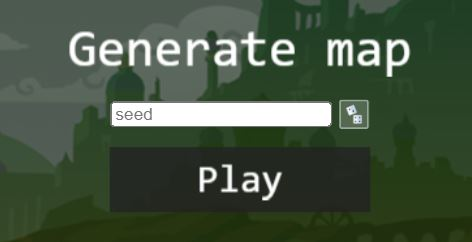
\includegraphics[scale=0.8]{kepek/jatekHasznalat/fomenu}
			\caption{Illusztráció a játék főmenüjéből}
			\label{fig:jatekHasznalat:fomenu}
		\end{figure}
		
		A játék megkezdése után egy másik képernyőn találjuk magunkat, amelyen különféle elemeket láthatunk. Egy példát erre \aref{fig:jatekHasznalat:game_scene} ábrán tekinthetünk meg. Itt különböző tájelemek helyezkednek el, kráterek, fák, és sima fűvel borított területek, ezenkívül pedig egy útvonal. 
		
		\begin{figure}[h!]
			\centering
			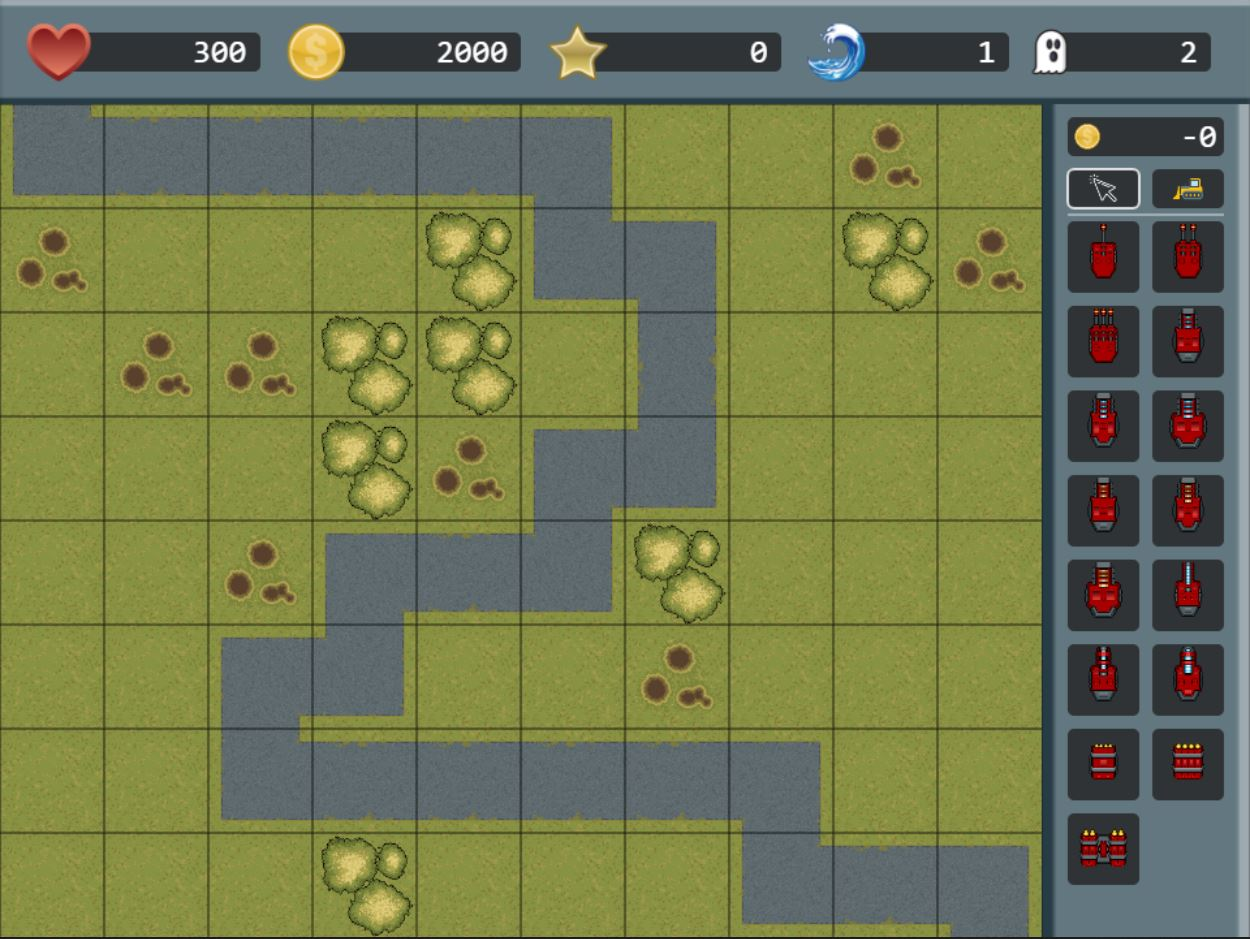
\includegraphics[scale=0.57]{kepek/jatekHasznalat/game_scene}
			\caption{A játék közvetlenül elindítás után}
			\label{fig:jatekHasznalat:game_scene}
		\end{figure}
		
		Az úton szörnyek (lásd: \myref{fig:jatekHasznalat:szorny} ábra) fognak elindulni, pár másodperccel a játék elindítása után, és megpróbálnak végigmenni rajta. A feladatunk az, hogy megakadályozzuk őket ebben. Ezt úgy tudjuk megtenni, hogy különféle tornyokat helyezünk le, ezek fogják sebezni a szörnyeket.
		Az ellenségek feje fölött egy-egy zöld csík látható, amikor megjelennek, ez az életüket szimbolizálja. Amennyiben sebzést szenvednek el, a zöld rész egyre kisebb lesz, amikor pedig teljesen elfogy, a szörny meghal. Az ellenfelek hullámokban, avagy hordaként érkeznek. Minden hullámmal egyre több, és erősebb ellenség fog érkezni.
		
		\begin{figure}[h!]
			\centering
			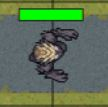
\includegraphics[scale=1.6]{kepek/jatekHasznalat/szorny}
			\caption{A legyőzendő ellenség}
			\label{fig:jatekHasznalat:szorny}
		\end{figure}
		
		Tornyokat csak üres, füves területekre tudunk építeni. Amennyiben nincs már hely ahova tudnánk tenni, le is rombolhatunk előzőleg épülteket, vagy pedig a tájelemeket is. Ezt a jobb oldalt látható felület által tehetjük meg (lásd: \myref{fig:jatekHasznalat:game_scene} ábra jobb oldala).		
		A játék kezdetekor az egér ikont ábrázoló gomb van kijelölve, ekkor ha egy már megépült toronyra rávisszük a kurzort, akkor látni fogunk egy kört körülötte. Ezen a körön belüli távolságra lévő ellenfeleket képes elérni a torony. Ez az egér ikonnal ellátott gomb tehát az úgynevezett "kijelölés mód", ha ezen a módon belül vagyunk, tehát ez a gomb van bekeretezve fehér színnel, akkor egyes objektumokra kattintva a játékon belül nem történik semmi, szimplán amelyik mező felett van a kurzorunk, az lesz kijelölve.
		Az ettől jobbra található, sárga buldózer ábrával ellátott gombra kattintva pedig az "eltávolító mód"-ba kerülünk. Ha ebben a módban vagyunk, és odamozgatjuk a kurzort (kattintás nélkül) egy-egy tárgyra a játékfelületen belül, akkor amíg az adott tárgy fölött van az egerünk, addig az előbb említett gombok feletti rubrikában látható, hogy amennyiben le szeretnénk rombolni az adott objektumot, milyen összeggel változna a pénzünk, avagy aranyunk. Az objektum tényleges eltávolítása kattintásra történik meg.
		Abban az esetben, ha egy korábban megépített tornyot szeretnénk megsemmisíteni, a torony eredeti értékének 60\%-át kapjuk vissza, tehát például ha egy toronyért 1000 aranyat fizettünk, amikor rávisszük a kurzort eltávolító módban, "+600"-at fogunk látni a rubrikában, tehát 600 aranyat kapunk vissza, a rombolás után. Ellenben kráter, vagy fa eltávolításához fizetnünk kell a rombolásért, tehát egy mínusz jel után fog megjelenni az összeg, amennyibe kerül.
		A két gomb alatti felületen különféle tornyok helyezkednek el, 5 különböző típusú toronyot tudunk építeni, és mind az 5 típusból létezik 3 különböző erősségű.
		A tornyok balról jobbra vannak sorbarendezve, tehát adott típusú toronynak először a leggyengébb változát láthatjuk, a végén pedig a legerősebbet, de összességében szituációfüggő is, hogy épp melyik az, amit a legjobban megéri építenünk. Az azonos típusú tornyok hasonló megjelenéssel rendelkeznek, hogy látható legyen az, hogy egy ugyanazon típuson belül helyezkednek el, az áruk azonban különböző.
		
		Az egyes tornyok tulajdonságairól részletes leírás alább, a fejezet végén lévő táblázatokban olvasható.(lásd: \myref{tab:torony_tipus_0}, \myref{tab:torony_tipus_1}, \myref{tab:torony_tipus_2}, \myref{tab:torony_tipus_3}, \myref{tab:torony_tipus_4})
		
		% TODO mindegyik torony - táblázat, a torony képével, képességeivel, árával stb.
		% TODO Tűzgyorsaság (lövés/sec) a lövés / sec az nem igazán hangzik érthetőnek mert több száz az érték és alig lő 2-t  ->2 lövés között 1000/firerate-nyit vár 
		% TODO effekt képességhez - Beletenni a PENETRATION-t  -> átütőképesség
		
	
		A felső felhasználói felületen (lásd \myref{fig:jatekHasznalat:felso_ui} ábra) balról jobbra haladva, a következőket láthatjuk:
		
		\begin{figure}[h!]
			\centering
			
\includegraphics[scale=0.575]{kepek/jatekHasznalat/felso_ui}
			\caption{A felülső felhasználói felület (UI) }
			\label{fig:jatekHasznalat:felso_ui}
		\end{figure}
		
		\begin{itemize}
			\item Piros szív ábra: Az itt látható szám az aktuális életünket jelzi. Ez csökkenni fog, ha egy szörnyet engedünk végigmenni az egész úton. Amikor teljesen elfogy, akkor veszítünk, az adott játék véget ér.
			
			\item Sárga érme "\$" jellel: Ebben a rubrikában az aktuális aranyunk jelenik meg. Ez az érték többször is változhat a játék során. Például toronyépítéskor levonódik a torony összege, ellenben amikor megölünk egy szörnyet akkor kapunk érte adott aranymennyiséget.
			
			\item Csillag ikon: A pillanatnyi összpontszámunkat mutatja. Minden ellenfél megölése után kapunk adott mennyiségű pontot. A végeredményként elért összpontszámot a játék vége után is megtekinthetjuk, mielőtt visszalépünk a főmenübe.
			
			\item Hullám: Azt jelzi, hogy hányadik beérkező hordánál, szörnyhullámnál tartunk éppen.
			
			\item Szellem ikon: A szörnyeket jelképezi. Azt jelzi a játékos számra, hogy az adott hullámban mennyi ellenség érkezik.
		\end{itemize}
	
		A fentieken kívül még megemlítendő, hogy amennyiben olyan tevékenységet kívánunk tenni, amely nem lehetséges az adott mezőben, (például nincs elég pénzünk, hogy megvegyük a jobb oldali menüből kiválasztott tornyot, vagy mondjuk ha az utat próbáljuk meg eltávolítani), úgy a mező pirosas színre vált, ha pedig lehetséges az akció végrehajtása, akkor élénk zöldes árnyalatot kap. (\Aref{fig:jatekHasznalat:kijeloles_minta}. ábrán bal oldalt az előbbi, jobb oldalt pedig az utóbbi látható.)
		
		\begin{figure}[h!]
			\centering
			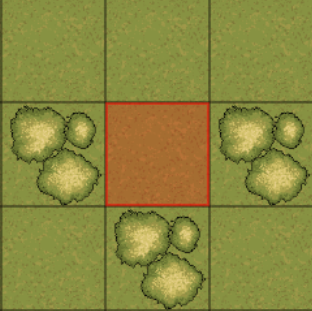
\includegraphics[scale=0.848]{kepek/jatekHasznalat/minta_rossz_kijeloles}
			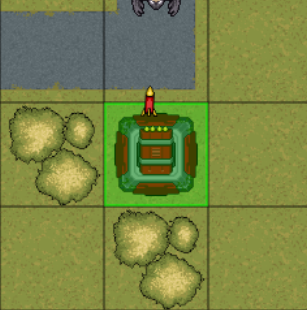
\includegraphics[scale=0.85]{kepek/jatekHasznalat/minta_jo_kijeloles}
			\caption{Minta kijelölésekre - lehetetlen, illetve teljesíthető akciók esetén}
			\label{fig:jatekHasznalat:kijeloles_minta}
		\end{figure}
		
		% game over scene
		
		Most, hogy elolvastuk az előbbieket, már mindent tudunk a játékmenetről. Ami tehát még hátravan, az az, hogy mi történik akkor, amikor esetlegesen elveszítjük az összes életünket, ezáltal a játékot is.
		Ekkor egy új felület jelenik meg előttünk (lásd: \myref{fig:jatekHasznalat:game_over_scene} ábra), amelyen egy "Game Over" felirat taláható, emellett itt megtekinthetjük a játék során elért összpontszámunkat, valamint a "Back to Main Menu" gombra kattintva pedig újra a főmenübe navigálhatjuk magunkat, hogy belekezdhessünk egy új játékmenetbe.
		
		\begin{figure}[h!]
			\centering
			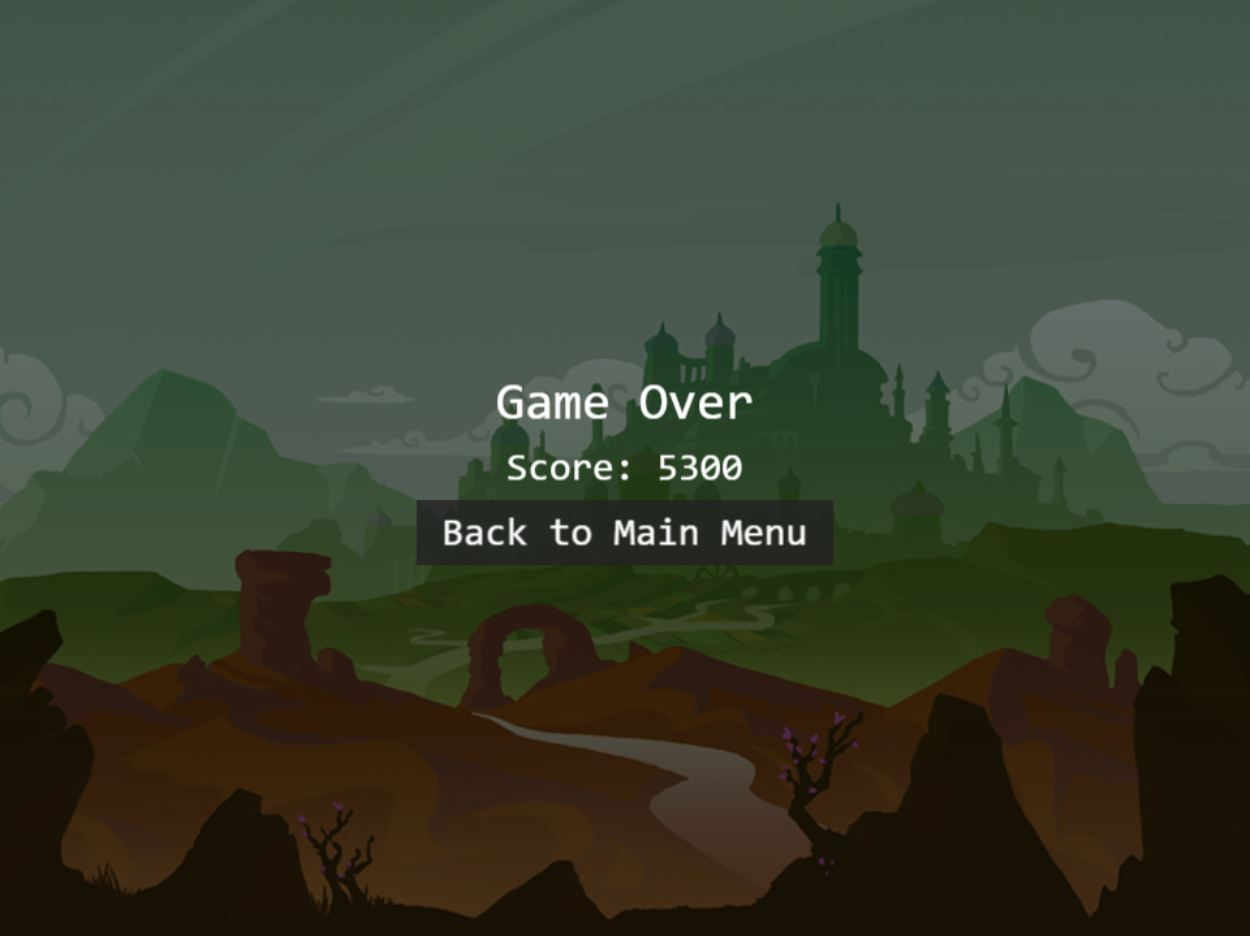
\includegraphics[scale=0.6]{kepek/jatekHasznalat/game_over_scene}
			\caption{Részlet a Game Over képernyőről}
			\label{fig:jatekHasznalat:game_over_scene}
		\end{figure}
	
		\begin{table}[h]
			\centering
			\caption{Első toronytípus tulajdonságai}
			\label{tab:torony_tipus_0}
			\begin{tabular}{|l|c|c|c|}
				\hline
				Kinézet & 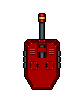
\includegraphics[scale=1.1]{kepek/jatekHasznalat/torony_01} & 
\includegraphics[scale=1.1]{kepek/jatekHasznalat/torony_02} & 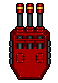
\includegraphics[scale=1.1]{kepek/jatekHasznalat/torony_03} \\ \hline
				Ár (arany) & 500 & 1200 & 3000 \\ \hline
				Maximum lövéstávolság & 220 & 250 & 280 \\ \hline
				Lövés/sec & 2 & 1.6 & 1.4 \\ \hline
				Sebzés & 25 & 25 & 25 \\ \hline
				% Százalékos sebzés & Nincs & Nincs & Nincs \\ \hline
				Képesség, effekt & \begin{tabular}{@{}c@{}}Egy lövésnél \\ 1 lövedéket lő ki.\end{tabular} & \begin{tabular}{@{}c@{}}Egy lövésnél \\ 2 lövedéket lő ki.\end{tabular} & \begin{tabular}{@{}c@{}}Egy lövésnél \\ 3 lövedéket lő ki.\end{tabular} \\ \hline
			\end{tabular}
		\end{table}
		
		\begin{table}[h]
			\centering
			\caption{Második toronytípus tulajdonságai}
			\label{tab:torony_tipus_1}
			\begin{tabular}{|l|c|c|c|}
				\hline
				Kinézet &  &  &  \\ \hline
				Ár (arany) & 800 & 1600 & 3200 \\ \hline
				Maximum lövéstávolság & 220 & 250 & 280 \\ \hline
				Lövés/sec & 1.4 & 1.4 & 1.4 \\ \hline
				Sebzés & 10 & 10 & 10 \\ \hline
				% Százalékos sebzés & Nincs & Nincs & Nincs \\ \hline
				Képesség, effekt & \begin{tabular}{@{}c@{}}Lassító \\ lövedéket lő ki.\end{tabular} & \begin{tabular}{@{}c@{}}1-es átütő- \\ képességű lassító \\ lövedéket lő ki.\end{tabular} & \begin{tabular}{@{}c@{}}2-es átütő- \\ képességű lassító \\ lövedéket lő ki.\end{tabular} \\ \hline
			\end{tabular}
		\end{table}
	
		\begin{table}[h]
			\centering
			\caption{Harmadik toronytípus tulajdonságai}
			\label{tab:torony_tipus_2}
			\begin{tabular}{|l|c|c|c|}
				\hline
				Kinézet &  &  &  \\ \hline
				Ár (arany) & 800 & 1600 & 3200 \\ \hline
				Maximum lövéstávolság & 220 & 250 & 280 \\ \hline
				Lövés/sec & 1.4 & 1.4 & 1.4 \\ \hline
				Sebzés & 10 & 10 & 10 \\ \hline
				% Százalékos sebzés & Nincs & Nincs & Nincs \\ \hline
				Képesség, effekt & \begin{tabular}{@{}c@{}}Tüzes lövedéket \\ lő ki. (DOT-ként)\end{tabular} & \begin{tabular}{@{}c@{}}1-es átütő- \\ képességű tüzes \\ lövedéket lő ki.\end{tabular} & \begin{tabular}{@{}c@{}}2-es átütő- \\ képességű tüzes \\ lövedéket lő ki.\end{tabular} \\ \hline
			\end{tabular}
		\end{table}
	
		%\begin{remark}
		%	Ez egy megjegyzés
		%\end{remark}
		%\footnotetext{DOT: Damage Over Time, magyarul olyan sebzésforma, amely nem egyszer sebez, hanem bizonyos időn keresztül folyamatosan sebzi az ellenfelet.}
	
		\begin{table}[h]
			\centering
			\caption{Negyedik toronytípus tulajdonságai}
			\label{tab:torony_tipus_3}
			\begin{tabular}{|l|c|c|c|}
				\hline
				Kinézet &  &  &  \\ \hline
				Ár (arany) & 700 & 1400 & 2800 \\ \hline
				Maximum lövéstávolság & 220 & 250 & 280 \\ \hline
				Lövés/sec & 1.4 & 1.6 & 2.0 \\ \hline
				% Sebzés & 0 & 0 & 0 \\ \hline
				Százalékos sebzés & 20 \% & 20 \% & 20 \% \\ \hline
				Képesség, effekt & \multicolumn{3}{c|}{Instant sebez, egyszerre egy ellenséget, lézersugárral.} \\ \hline
			\end{tabular}
		\end{table}
	
		\begin{table}[h]
			\centering
			\caption{Ötödik toronytípus tulajdonságai}
			\label{tab:torony_tipus_4}
			\begin{tabular}{|l|c|c|c|}
				\hline
				Kinézet &  &  &  \\ \hline
				Ár (arany) & 1000 & 2500 & 4000 \\ \hline
				Maximum lövéstávolság & 220 & 250 & 280 \\ \hline
				Lövés/sec & 1.0 & 1.05 & 1.1 \\ \hline
				Sebzés & 10 & 10 & 10 \\ \hline
				Százalékos sebzés & 10 \% & 10 \% & 10 \% \\ \hline
				Képesség, effekt & \multicolumn{3}{c|}{\begin{tabular}{@{}c@{}}Rakétát lő ki, becsapódáskor a robbanás \\ hatósugarában tartózkodó összes ellenfelet sebzi.\end{tabular}} \\ \hline
				Robbanás hatósugara & 50 & 75 & 100 \\ \hline
			\end{tabular}
		\end{table}
	
	\end{MySection}

\end{MyChapter}